\documentclass[journal]{IEEEtran}

\PassOptionsToPackage{hyphens}{url}
\usepackage{amsmath,amssymb,amsfonts}
\usepackage{mathtools}
\usepackage{amsthm}
\newtheorem{lemma}{Lemma}
\usepackage{algorithm}
\usepackage{algorithmic}
\usepackage{graphicx}
\usepackage{textcomp}
\usepackage{booktabs}
\usepackage{multirow}
\usepackage{tikz}
\usetikzlibrary{arrows.meta,positioning,shapes.geometric,shapes.symbols,calc,fit,backgrounds}
\usepackage{url}
\usepackage[hidelinks]{hyperref}

\graphicspath{{../results/figures/}{figures/}}
% Auto-generated by code/emit_macros.py -- do not edit by hand.
\newcommand{\Cm}{4}
\newcommand{\Cnt}{139}
\newcommand{\Cntot}{140}
\newcommand{\CssaTraj}{200{,}000}
\newcommand{\Cmttd}{3.64}
\newcommand{\Cmresp}{0.31}
\newcommand{\Cmttr}{3.94}
\newcommand{\Cebreach}{0.57}
\newcommand{\Cedenial}{0.39}
\newcommand{\Cedataloss}{0.38}
\newcommand{\Cexposure}{2.50}
\newcommand{\Cresdev}{0.21}
\newcommand{\Csigstar}{2.17}
\newcommand{\Ctaustar}{32}
\newcommand{\CJstar}{1.92}
\newcommand{\CSstar}{0.97}
\newcommand{\COstar}{0.95}
\newcommand{\Cdenialstar}{0.15}
\newcommand{\Cdatalossstar}{0.30}
\newcommand{\Cdenialdroppct}{62}
\newcommand{\Cblindtau}{25}
\newcommand{\Cblindpen}{14}
\newcommand{\CmLo}{2}
\newcommand{\CmHi}{6}
\newcommand{\CntLo}{29}
\newcommand{\CntHi}{419}
\newcommand{\CbreachLo}{0.54}
\newcommand{\CbreachHi}{0.57}
\newcommand{\CsensTop}{wL}
\newcommand{\CcovMttrPct}{21}
\newcommand{\CcovLossPct}{43}
\newcommand{\CpeakDenPct}{7.5}
\newcommand{\CpeakDenT}{3.2}
\newcommand{\CminAvailPct}{98.0}
\newcommand{\CmttdStar}{3.32}
\newcommand{\CexfilDropPct}{32}
\newcommand{\ClossDropPct}{23}


\newcommand{\E}{\mathbb{E}}
\newcommand{\Prob}{\mathbb{P}}
\DeclareMathOperator*{\argmin}{arg\,min}

\begin{document}

\title{CRADLE: Transient Security and Dependability Analysis of
Crypto-Ransomware Kill-Chains in MEC Micro-Datacenters under Footprint-Aware
Detection and Backup-Restore Defense}

\author{Tuan~Anh~Nguyen%
\thanks{T.~A.~Nguyen is with the Faculty of Information Technology, Ho Chi Minh
City University of Industry and Trade (HUIT), Ho Chi Minh City, Vietnam
(e-mail: anhngt@huit.edu.vn).}%
\thanks{All models, solvers, the simulator, and the scripts regenerating every
figure, table and in-text number are openly available at
\url{https://github.com/anhnt2407/273-CRADLE-Transient-Ransomware-Kill-Chain-Detection-Backup-Restore-MEC-Micro-Datacenter-SRN}.}}

\markboth{IEEE Transactions on Dependable and Secure Computing (submitted)}%
{Nguyen: Transient Security and Dependability of Ransomware Kill-Chains in MEC Micro-Datacenters}

\maketitle

\begin{abstract}
Multi-access edge computing places a small number of virtualized servers beside
base stations, and such micro-datacenters face crypto-ransomware campaigns of
growing severity. A ransomware incident differs from a classical breach because
locked servers remain restorable from immutable backups. The true cost of an
incident becomes the transient loss of confidentiality, service availability and
data recency accrued during the race between the attacker kill-chain and the
defender response. The present work develops CRADLE, a continuous-time Markov
reward model drawn as a stochastic reward net, of an ordered compromise,
exfiltration, encryption and lock kill-chain on a micro-datacenter. The defense
combines an endpoint monitor whose detection hazard grows with the encryption
and exfiltration footprint and an isolate-and-restore response with explicit
recovery-point and recovery-time semantics. The model delivers transient state
probabilities, accumulated-reward security losses, first-passage detection and
resolution distributions, and closed per-incident expectations from the
fundamental matrix. A proof establishes a structural departure, under which
footprint-aware detection breaks the memoryless recovery law of prior
uniform-recovery models. A defender co-design procedure tunes detection
sensitivity and backup cadence jointly along a security-versus-spend Pareto
frontier. An independent Gillespie simulation validates every analytic result,
and the numerical evidence gives actionable guidance for edge ransomware
resilience.
\end{abstract}

\begin{IEEEkeywords}
Multi-access edge computing, ransomware, kill-chain, stochastic reward nets,
continuous-time Markov chains, transient analysis, dependability, security,
backup and restore, performability.
\end{IEEEkeywords}

% ======================================================================= %
\section{Introduction}
\IEEEPARstart{M}{ulti-access} edge computing (MEC) pushes computation to
micro-datacenters (MEDCs) of a few virtualized servers placed beside base
stations, and the resulting proximity delivers the low latency demanded by
immersive, industrial and vehicular applications~\cite{mao2017survey,taleb2017mec}.
Such proximity creates a substantial attack surface at the same time. An MEDC
occupies a physically and administratively exposed location, hosts multi-tenant
virtual machines and containers, and forms a natural staging point for
adversaries seeking the data and the control flows traversing the
edge~\cite{roman2018survey}. The dominant monetized threat against such edge
fleets today is crypto-ransomware. An adversary gains an initial foothold, moves laterally
between servers, exfiltrates data for double-extortion leverage, and then
encrypts data at rest to deny service until a ransom is
paid~\cite{kharraz2015gordian,alrimy2018ransomware,razaulla2023age}.

Quantitative stochastic models have proven invaluable for reasoning about the
security and the dependability of computing systems before deployment. The
MEDC-under-attack model of Liu \emph{et al.}~\cite{liu2021transient} is the
closest antecedent. The antecedent analyses a lateral-movement campaign on an
MEDC as an absorbing continuous-time Markov chain (CTMC) and computes transient
infection, exfiltration and loss metrics. Two simplifications of the antecedent
model matter a great deal for ransomware. First, recovery is a single uniform rate to an absorbing
state in which defensive mechanisms have been deployed, and the rate carries no
dependence on the progress of the attack, which makes the recovery probability
exactly memoryless. Detection in practice is driven by the noise of the attacker
because encryption produces a high-entropy input-output storm and mass data
egress, and an endpoint monitor observes such activity precisely because the
campaign is advancing. Second, the antecedent carries no notion of data-at-rest
denial and of the reversal of such denial. Encryption is absent as a recoverable
service-denial state, and no backup-and-restore layer supplies recovery-point or
recovery-time semantics, which are exactly the levers under defender control.

The present work closes the gap left by the antecedent model. We propose CRADLE,
a transient Markov reward model expressed as a stochastic reward net (SRN), of a
crypto-ransomware double-extortion kill-chain on an MEDC, defended by a
footprint-aware endpoint detection-and-response (EDR) monitor and by an
immutable-backup isolate-and-restore response. A ransomware incident inside the
CRADLE model remains survivable by construction. Every trajectory eventually
reaches a restored condition, and the object of study becomes the transient
security and dependability loss in confidentiality, service availability, data
recency and downtime accumulated while the kill-chain races the response.

The main contributions of the present study appear in the following list.
\begin{itemize}
\item An ordered double-extortion ransomware SRN (Section~\ref{sec:model}) whose
per-server kill-chain runs from vulnerable to compromised, to exfiltrating, to
encrypting and to locked, with lateral movement scaling in the active footprint,
and in which encryption becomes a recoverable service-denial state rather than
an absorbing breach.
\item A footprint-aware detection hazard keyed on the encryption and
exfiltration input-output footprint, coupled to an isolate-and-restore response
with explicit recovery-point and recovery-time semantics and with imperfect
restore coverage (Section~\ref{sec:model}). We prove the coupling breaks the
memoryless recovery law of uniform-recovery models, and the resolution curve
takes an S shape instead of an exponential shape.
\item Exact transient and per-incident measures (Section~\ref{sec:measures}),
namely transient probabilities and accumulated-reward losses through matrix
exponentials, first-passage detection and resolution distributions, and closed
per-incident expectations through the fundamental matrix.
\item A defender co-design algorithm (Section~\ref{sec:measures}) optimizing
detection sensitivity and backup cadence jointly to minimize expected total
cost, tracing the security-versus-spend Pareto frontier and quantifying the
penalty of a detection-blind backup schedule.
\item A dual analytic and simulation validation plus a numerical study
(Section~\ref{sec:results}) surfacing actionable design guidance, including the
counterintuitive result under which sharper detection lets a defender back up
less often.
\end{itemize}

% ======================================================================= %
\section{Related Work}\label{sec:related}
\subsection{Stochastic dependability and security modelling}
Markov reward models, stochastic Petri and reward nets, and semi-Markov
processes are the standard vehicles for quantifying availability, reliability
and security of computing systems~\cite{trivedi2016probability,
trivedi2017reliability,nicol2004modelbased,ciardo1992srn}. Meyer introduced
performability as the joint treatment of performance and
dependability~\cite{meyer1980performability}, and Nicol \emph{et al.} extended
model-based evaluation from dependability toward quantitative
security~\cite{nicol2004modelbased}. The dependability and security taxonomy of
Avi\v{z}ienis \emph{et al.}~\cite{avizienis2004basic} defines integrity and
availability as distinct attributes, and encryption-based denial affects both
attributes at once through a fault whose handling combines detection, isolation
and recovery. Intrusion-tolerance models in the same lineage, for instance the
state-transition security model of Madan \emph{et al.}~\cite{madan2004method},
derive a mean time to security failure from a semi-Markov process with
absorbing states. Our study lifts the reward-based and first-passage-based
measures of such models from a single host to a footprint-coupled MEDC fleet
with data-centric restore.

\subsection{Edge micro-datacenters under attack}
Liu \emph{et al.}~\cite{liu2021transient} model a lateral-movement attack on an
MEDC as an absorbing CTMC with a uniform recovery rate into a good state, and
the model serves as our direct antecedent and baseline. Roman \emph{et
al.}~\cite{roman2018survey} survey the threat landscape of edge and fog
deployments and motivate the exposure assumptions of our threat model. CRADLE
differs from the antecedent in threat model and in objective. Our detection
hazard is keyed on the encryption and exfiltration footprint rather than on the
compromised-node count. Encryption becomes a recoverable denial state rather
than a terminal breach. Our response is a backup restore with recovery-point
and recovery-time economics rather than a re-image.

\subsection{Ransomware behaviour and defenses}
Empirical and systems work dissects ransomware behaviour and the defenses
against ransomware, covering file-system self-healing, real-time write
monitoring and behavioural detection~\cite{kharraz2015gordian,
continella2016shieldfs,kharraz2017redemption,beaman2021ransomware}. Early
comparative analyses of ransomware families document the cryptographic
machinery underlying data denial~\cite{gazet2010comparative}, and the
commoditized crimeware market explains the scale of modern
campaigns~\cite{sood2013crimeware}. Surveys of ransomware evolution record the
shift toward double extortion, under which an operator exfiltrates data before
encryption and threatens public release~\cite{razaulla2023age,
alrimy2018ransomware}. Studies of advanced persistent threats describe the
lateral-movement stages preceding the final payload~\cite{ussath2016apt}. The
listed studies are measurement and mechanism studies, and no prior transient
Markov reward model captures the exfiltrate-then-encrypt kill-chain in
combination with detection and backup-restore economics.

\subsection{Proactive recovery and storage dependability}
Moving-target defense and rejuvenation-based recovery reset attacker progress on
a timer or on a trigger~\cite{jajodia2011mtd,huang1995rejuvenation}. Our restore
is conceptually a triggered reset, and the restore remains data-centric because
the restored object is encrypted data drawn from an immutable backup and the
residual cost is the recovery point. Storage dependability frameworks evaluate
backup and mirroring designs against financial
objectives~\cite{keeton2004framework}, and CRADLE embeds a comparable
cost-driven choice inside a live adversarial race.

\subsection{Numerical methods}
We use the matrix exponential for transient solutions, Jensen uniformization as
an independent cross-check~\cite{reibman1988transient}, a Van Loan style
augmented exponential for accumulated
rewards~\cite{vanloan1978,moler2003nineteen}, the fundamental matrix for
per-incident expectations, phase-type arguments for the first-passage
law~\cite{latouche1999matrix}, and the exact stochastic simulation algorithm of
Gillespie for validation~\cite{gillespie1977exact}.

% ======================================================================= %
\section{Architecture, Threat Model and Stochastic Reward Net}\label{sec:model}

\subsection{Architecture}
Fig.~\ref{fig:arch} depicts the deployment and the two defensive planes of the
system. An MEDC hosts a fixed number of MEC
servers behind one or more base stations, and each server runs a virtualization
stack instantiating tenant services close to endpoint and cyber-physical
devices. Two independent defensive planes overlay the compute fabric of the
micro-datacenter. An EDR monitor
continuously observes host and network telemetry, and the alert hazard of the
monitor rises with the volume of ransomware-indicative activity such as
high-entropy write bursts from encryption and anomalous data egress from
exfiltration. An immutable-backup subsystem periodically snapshots server data
to write-once storage. Upon an incident the subsystem drives an
isolate-and-restore response, which network-isolates the MEDC and restores
servers from the last good snapshot.

\begin{figure}[t]
\centering
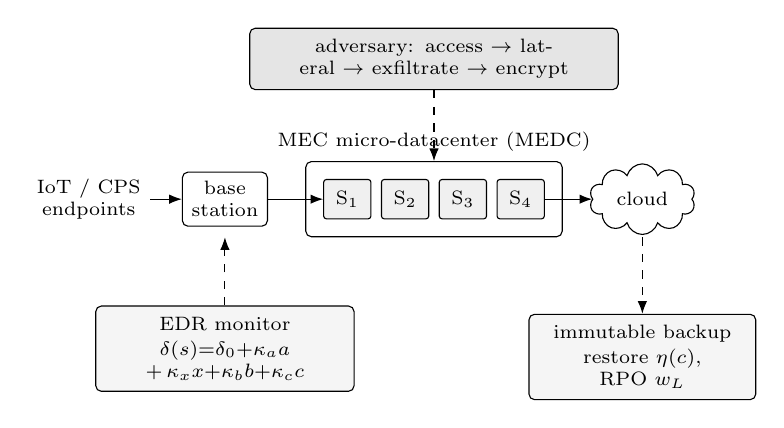
\begin{tikzpicture}[font=\scriptsize,
  srv/.style={draw,rounded corners=1pt,minimum width=6mm,minimum height=5mm,fill=black!6},
  box/.style={draw,rounded corners=2pt,inner sep=2.2mm},
  plane/.style={draw,rounded corners=2pt,align=center,inner sep=1.4mm,fill=black!4},
  adv/.style={draw,rounded corners=2pt,fill=black!10,align=center,inner sep=1.4mm,text width=44mm},
  ar/.style={-{Latex[length=1.6mm]}}]
% devices
\node (dev) [align=center] {IoT / CPS\\endpoints};
\node (bs) [draw,rounded corners=2pt,right=4mm of dev,align=center] {base\\station};
% MEDC box with m servers
\node (s1) [srv,right=7mm of bs] {S$_1$};
\node (s2) [srv,right=1.2mm of s1] {S$_2$};
\node (s3) [srv,right=1.2mm of s2] {S$_3$};
\node (s4) [srv,right=1.2mm of s3] {S$_4$};
\begin{scope}[on background layer]
\node (medc) [box,fit=(s1)(s4),label=above:{MEC micro-datacenter (MEDC)}] {};
\end{scope}
\node (cloud) [draw,cloud,aspect=2,right=6mm of s4,minimum width=12mm] {cloud};
% adversary
\node (att) [adv,above=9mm of medc.north]
  {adversary: access $\to$ lateral $\to$ exfiltrate $\to$ encrypt};
% defensive planes
\node (edr) [plane,text width=30mm,anchor=north] at ([yshift=-10mm]bs.south)
  {EDR monitor\\[1pt] $\delta(s){=}\delta_0{+}\kappa_a a$\\$
   {+}\,\kappa_x x{+}\kappa_b b{+}\kappa_c c$};
\node (bkp) [plane,text width=26mm,anchor=north] at ([yshift=-10mm]cloud.south)
  {immutable backup\\[1pt] restore $\eta(c)$, RPO $w_L$};
% arrows
\draw[ar] (dev)--(bs); \draw[ar] (bs)--(s1.west|-bs); \draw[ar] (s4)--(cloud);
\draw[ar,dashed] (att.south)--(medc.north);
\draw[ar,dashed] (edr.north)--(edr.north|-medc.south);
\draw[ar,dashed] (bkp.north|-medc.south)--(bkp.north);
\end{tikzpicture}
\caption{CRADLE system architecture.}
\label{fig:arch}
\end{figure}

\subsection{Threat model}
The adversary follows a ransomware double-extortion kill-chain. The adversary
obtains initial access to one server and then propagates laterally, and the
propagation accelerates with the number of controlled servers. On a controlled
server the adversary exfiltrates data, which creates confidentiality loss and
extortion leverage, and only afterwards encrypts the same data until the server
reaches a locked condition denying service. The defender remains unaware of the
campaign until the EDR monitor fires, detection remains imperfect, and the
timeliness of detection depends on the attacker footprint. We assume network
isolation becomes effective once triggered, and isolation halts further spread
and egress. Host-local encryption already in flight may complete before the end
of the restore.
Immutable backups are not corruptible, which is a design goal of modern
write-once backup. We exclude the ransom-payment decision by design, because
CRADLE is a defender-side resilience model built on a restore-not-pay premise.

\subsection{State space}
The MEDC holds a fixed number of servers, and every server occupies exactly one
kill-chain stage. A transient operational state is the tuple
\begin{equation}
s=(a,x,b,c,d),
\end{equation}
in which the first four entries count servers in the compromised, exfiltrating,
encrypting and locked stages, and the last entry indexes the campaign phase with
value zero for stealth and value one for response. The count of clean vulnerable
servers, the campaign footprint and the active non-locked foothold follow from
\begin{equation}
p=a+x+b+c,\qquad V=m-p,\qquad h=a+x+b.
\label{eq:counts}
\end{equation}
Validity requires non-negative counts and a footprint no larger than the fleet
size. The stealth phase exists for every lattice point, and the response phase
exists only for a non-empty footprint, because a campaign must exist before the
start of a response. A single absorbing state denoted \textsc{Good} represents
the fully restored and incident-resolved MEDC.
Table~\ref{tab:states} summarizes the encoding of every symbol and the
corresponding service condition. Counting the two phases gives the size of the
transient state set,
\begin{equation}
|\mathcal{S}|=2\binom{m+4}{4}-1,
\label{eq:ssize}
\end{equation}
which amounts to \Cnt{} transient states plus one absorbing state for the base
case of \Cm{} servers.

\begin{table}[t]
\caption{State encoding.}
\label{tab:states}
\centering\footnotesize
\begin{tabular}{@{}clc@{}}
\toprule
symbol & meaning & service\\
\midrule
$V=m-p$ & Vulnerable (clean, serving) & up\\
$a$ & Compromised (foothold, staging) & up\\
$x$ & Exfiltrating (data egress in progress) & up (leaking)\\
$b$ & Encrypting (crypto in progress) & degraded\\
$c$ & Locked (data denied) & down\\
$d$ & phase: $0$ stealth / $1$ response & --\\
$\textsc{Good}$ & restored (absorbing) & up\\
\bottomrule
\end{tabular}
\end{table}

\subsection{Transition rules}
Fig.~\ref{fig:srn} shows the kill-chain and the phase automaton, and the
aggregate rate laws appear in Table~\ref{tab:trans}. In the stealth phase the
adversary first obtains a foothold on a clean MEDC at the initial-access rate. A
clean server afterwards becomes compromised through lateral movement at a rate
proportional to the active foothold, which reproduces the epidemic
footprint-scaling of the antecedent model~\cite{liu2021transient}. Every
compromised server begins exfiltration at a per-server onset rate. An
exfiltrating server completes one stolen dataset and only afterwards begins
encryption at a per-server completion rate. An encrypting server completes to
the locked stage at a per-server encryption rate. The campaign becomes detected,
and the phase index moves to the response value, at the footprint-aware hazard
\begin{equation}
\delta(s)=\delta_0+\kappa_a a+\kappa_x x+\kappa_b b+\kappa_c c,\qquad
\delta(s)\!=\!0 \text{ if } p{=}0,
\label{eq:delta}
\end{equation}
whose stage gains obey the strict ordering
\begin{equation}
\kappa_b>\kappa_c>\kappa_x\ge\kappa_a .
\label{eq:korder}
\end{equation}
An encrypting server sustains a high-entropy write storm and remains the loudest
live signal, a locked server raises a user-visible outage alarm, an exfiltrating
server leaves an egress signature, and a bare foothold stays nearly silent. In the response
phase network isolation halts lateral movement, exfiltration and new encryption
onsets. Host-local encryption already running completes at the same encryption
rate, and the restore fires to \textsc{Good} at the state-dependent rate
\begin{equation}
\eta(c)=\frac{1}{\mathrm{RTO}_0+\mathrm{RTO}_1\,c},
\label{eq:eta}
\end{equation}
under which the recovery time grows with the number of locked servers awaiting
restoration. With restore coverage in the unit interval, a complementary
fraction of restores are incomplete and leave a residual foothold, and the
campaign returns to a single compromised server.

\begin{figure}[t]
\centering
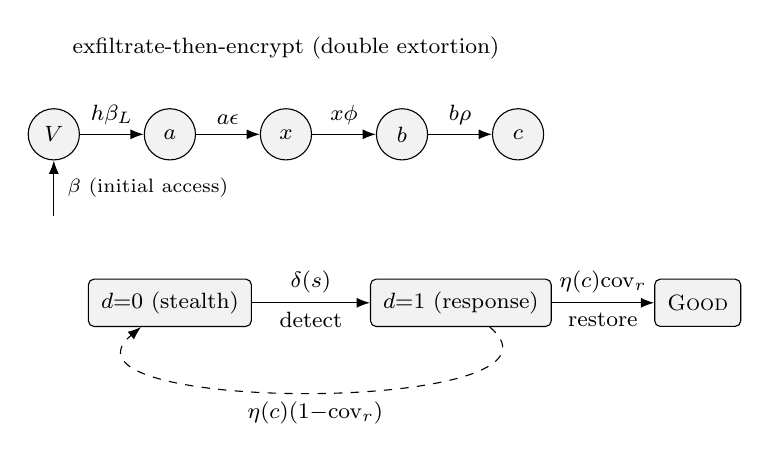
\begin{tikzpicture}[font=\footnotesize,>=Latex,node distance=8.1mm,
  st/.style={draw,circle,minimum size=6.5mm,inner sep=0pt,fill=black!5},
  ph/.style={draw,rounded corners=2pt,minimum height=6mm,inner sep=1.6mm,fill=black!5},
  ar/.style={->}]
% per-server kill chain
\node (V) [st] {$V$};
\node (A) [st,right=of V] {$a$};
\node (X) [st,right=of A] {$x$};
\node (B) [st,right=of X] {$b$};
\node (L) [st,right=of B] {$c$};
\draw[ar] (V)--(A) node[midway,above]{$h\beta_L$};
\draw[ar] (A)--(X) node[midway,above]{$a\epsilon$};
\draw[ar] (X)--(B) node[midway,above]{$x\phi$};
\draw[ar] (B)--(L) node[midway,above]{$b\rho$};
\draw[ar] ([yshift=-7mm]V.south) -- (V.south)
  node[midway,right=0.5mm,font=\scriptsize] {$\beta$ (initial access)};
\node[above=5mm of X] {exfiltrate-then-encrypt (double extortion)};
% phase automaton
\node (S0) [ph,below=15mm of A] {$d{=}0$ (stealth)};
\node (S1) [ph,right=15mm of S0] {$d{=}1$ (response)};
\node (G)  [ph,right=13mm of S1] {\textsc{Good}};
\draw[ar] (S0)--(S1) node[midway,above]{$\delta(s)$} node[midway,below]{detect};
\draw[ar] (S1)--(G)  node[midway,above]{$\eta(c)\mathrm{cov}_r$} node[midway,below]{restore};
\draw[ar,dashed] (S1) to[out=-40,in=-140]
  node[midway,below]{$\eta(c)(1{-}\mathrm{cov}_r)$} (S0);
\end{tikzpicture}
\caption{Kill-chain stages and campaign-phase automaton.}
\label{fig:srn}
\end{figure}

\begin{table}[t]
\caption{Transition rate laws.}
\label{tab:trans}
\centering\footnotesize
\setlength{\tabcolsep}{2pt}\scriptsize
\begin{tabular}{@{}lllc@{}}
\toprule
activity & effect & rate & guard\\
\midrule
initial access & $(0,0,0,0,0)\!\to\!(1,0,0,0,0)$ & $\beta$ & $p{=}0,d{=}0$\\
lateral move & $a\!\to\!a{+}1$ & $h\,\beta_L$ & $V{\ge}1,h{\ge}1,d{=}0$\\
exfil.\ onset & $a\!\to\!a{-}1,\,x\!\to\!x{+}1$ & $a\,\epsilon$ & $a{\ge}1,d{=}0$\\
exfil.\ done & $x\!\to\!x{-}1,\,b\!\to\!b{+}1$ & $x\,\phi$ & $x{\ge}1,d{=}0$\\
encrypt done & $b\!\to\!b{-}1,\,c\!\to\!c{+}1$ & $b\,\rho$ & $b{\ge}1$\\
detection & $d\!:\!0\!\to\!1$ & $\delta(s)$ & $p{\ge}1,d{=}0$\\
restore & $\to\textsc{Good}$ & $\eta(c)\,\mathrm{cov}_r$ & $d{=}1$\\
partial restore & $\to(1,0,0,0,0)$ & $\eta(c)(1{-}\mathrm{cov}_r)$ & $d{=}1$\\
\bottomrule
\end{tabular}

\end{table}

\subsection{Generator}
The transient state set collects every operational state, and a single absorbing
state completes the chain. The infinitesimal generator collects the arc rates
through
\begin{equation}
q_{s,s'}=\!\!\sum_{\text{arcs } s\to s'}\!\!\lambda,\qquad
q_{s,s}=-\!\!\sum_{s'\ne s}\!q_{s,s'},
\label{eq:gen}
\end{equation}
which drives every row sum of the generator to zero. The row of the absorbing
state contains only zero entries. Algorithm~\ref{alg:gen} synthesizes the generator
from the rate laws, and a numerical assertion confirms the row sums. Default
parameters per day appear in Table~\ref{tab:params}, and the chosen values place
the incident on a multi-day timescale in which detection, encryption and restore
genuinely compete.

\begin{table}[t]
\caption{Default parameters.}
\label{tab:params}
\centering\footnotesize
\begin{tabular}{@{}llrl@{}}
\toprule
symbol & meaning & default & unit\\
\midrule
$m$ & MEC servers in the MEDC & 4 & servers\\
$\beta$ & initial-access rate & 0.50 & d$^{-1}$\\
$\beta_L$ & lateral-movement rate / active foothold & 0.40 & d$^{-1}$\\
$\epsilon$ & exfiltration-onset rate / compromised & 0.80 & d$^{-1}$\\
$\phi$ & exfiltration-completion rate / exfiltrating & 1.00 & d$^{-1}$\\
$\rho$ & encryption-completion rate / encrypting & 2.00 & d$^{-1}$\\
$\delta_0$ & baseline detection hazard & 0.20 & d$^{-1}$\\
$\kappa_a$ & detection gain / compromised server & 0.00 & d$^{-1}$\\
$\kappa_x$ & detection gain / exfiltrating server & 0.50 & d$^{-1}$\\
$\kappa_b$ & detection gain / encrypting server & 1.50 & d$^{-1}$\\
$\kappa_c$ & detection gain / locked server & 0.80 & d$^{-1}$\\
$\mathrm{RTO}_0$ & base restore time & 0.25 & d\\
$\mathrm{RTO}_1$ & restore-time growth / locked server & 0.15 & d\\
$w_L$ & data loss / locked server (RPO) & 1.00 & unit\\
$\mathrm{cov}_r$ & restore coverage & 1.00 & --\\
\bottomrule
\end{tabular}

\end{table}

\begin{algorithm}[t]
\caption{CRADLE generator synthesis}
\label{alg:gen}
\begin{algorithmic}[1]
\REQUIRE parameters $\theta$, size $m$
\STATE enumerate $\mathcal{S}=\{(a,x,b,c,d): a{+}x{+}b{+}c\le m,\ d\in\{0,1\},\
(d{=}1\Rightarrow p\ge1)\}$
\STATE $Q\gets 0$
\FORALL{$s=(a,x,b,c,d)\in\mathcal{S}$}
  \FORALL{$(s',\lambda)$ in \textsc{Transitions}$(s;\theta)$ (Table~\ref{tab:trans})}
    \STATE $Q_{s,s'}\gets Q_{s,s'}+\lambda$,\quad $Q_{s,s}\gets Q_{s,s}-\lambda$
  \ENDFOR
\ENDFOR
\STATE \textbf{assert} $\max_s|\sum_{s'}Q_{s,s'}|<\varepsilon$
\RETURN $Q$
\end{algorithmic}
\end{algorithm}

% ======================================================================= %
\section{Measures, Solution and Defender Co-Design}\label{sec:measures}
The initial distribution places all mass on the clean state, and the transient
distribution obeys the matrix-exponential law
\begin{equation}
\pi(t)=\pi_0\,e^{Qt}.
\label{eq:transient}
\end{equation}

\subsection{Transient and accumulated measures}
The expected number of servers in a stage is a reward-weighted marginal of the
transient distribution. The expected available service fraction and the
probability of service denial both follow from the locked-server marginal,
\begin{equation}
\begin{aligned}
\E[c(t)]&=\sum_{s}c_s\,\pi_s(t),\qquad A(t)=1-\frac{\E[c(t)]}{m},\\
P_{\mathrm{dn}}(t)&=\Prob\!\left(c(t)\ge1\right).
\end{aligned}
\label{eq:marginals}
\end{equation}
For a given reward-rate vector the expected accumulated reward to a chosen time
horizon is obtained without quadrature from the
augmented exponential
\begin{equation}
\begin{bmatrix}\pi(t)\\ \Lambda(t)\end{bmatrix}
=\exp\!\left(\begin{bmatrix}Q^\top & 0\\ I & 0\end{bmatrix}t\right)
\begin{bmatrix}\pi_0\\ 0\end{bmatrix},\quad
L_r(t)=r^\top\Lambda(t).
\label{eq:accum}
\end{equation}
We instantiate the reward vector as the locked count for service-denial
server-days, as the exfiltration-completion flux restricted to the stealth phase
for stolen datasets, and as the restore flux weighted by the recovery point for
data lost at restore.

\subsection{First-passage distributions}
A trajectory remains stealthy exactly until detection, and the resolution event
coincides with absorption. Both first-passage distribution functions follow
directly from the transient distribution,
\begin{equation}
\begin{aligned}
\Prob(\text{detected}\le t)&=1-\!\!\sum_{s:d_s=0}\!\!\pi_s(t),\\
\Prob(\text{resolved}\le t)&=\pi_{\textsc{Good}}(t).
\end{aligned}
\label{eq:cdf}
\end{equation}

\subsection{Per-incident expectations}
Let the generator restricted to the transient states supply the fundamental
matrix. The expected sojourn vector before absorption satisfies
\begin{equation}
\tau^\top=\pi_{0,\mathcal{S}}^\top(-U)^{-1},
\label{eq:tau}
\end{equation}
and every per-incident total becomes a linear functional of the sojourn vector.
The expected total time spent in stealth states gives the mean time to detection,
the expected total time spent in response states gives the mean response
duration, and the sum of both quantities gives the mean time to resolution. The
same construction gives the expected number of exfiltrated datasets, the
expected denial server-days, and the expected data loss at restore. The additive
identity between the three time measures holds exactly, and a numerical check
confirms the identity to machine precision.

\subsection{Structural result}
In a uniform-recovery model every transient state exits to the absorbing state
at a single rate, and the resolution distribution function is exactly an
exponential distribution function. CRADLE behaves in a qualitatively different
manner, as the following statement makes precise.

\begin{lemma}[Non-memoryless resolution]\label{lem:nonexp}
Assume all rates of the generator are finite and assume the restore rate
$\eta(\cdot)$ is finite. Then the time to resolution $T_R$, defined as the first
passage from the clean state to \textnormal{\textsc{Good}}, is a phase-type random variable
whose density satisfies $f_{T_R}(0^+)=0$. Consequently $T_R$ is not
exponentially distributed, and the resolution distribution function is not of
the form $1-e^{-\gamma t}$ for any $\gamma>0$.
\end{lemma}
\begin{proof}
Absorption into \textsc{Good} occurs only from response states, and response
states are reachable only through the detection event, because no arc leads from
a stealth state directly to \textsc{Good}. Every path to absorption therefore
visits at least two distinct transient states, which gives $T_R\ge T_1+T_2$ with
$T_1$ the positive time to detection and $T_2$ the positive residual time to
restore. As a first passage in a finite CTMC starting from a single transient
state, $T_R$ is phase-type~\cite{latouche1999matrix}. At least two phases are
traversed with probability one, hence the density at the origin vanishes and
$f_{T_R}(0^+)=0$. The exponential density equals $\gamma e^{-\gamma t}$ with a
strictly positive value $\gamma$ at the origin, and $T_R$ cannot be exponential.
\end{proof}

The stealth window imprints an initial dead time on the resolution curve, which
produces the S shape. The coupling of detection to attack progress lies beyond
the representational reach of a uniform-recovery
model~\cite{liu2021transient}. Section~\ref{sec:results} quantifies the
departure from the exponential law in numerical terms.

\subsection{Security and dependability cost}
We weight the incident harms into a single security-dependability loss and add
the operational spend of the defender,
\begin{align}
S &= c_{\mathrm{br}}\E[\text{exfil}]+c_{\mathrm{dn}}\E[\text{denial}]\nonumber\\
  &\quad +c_{\mathrm{dl}}\E[\text{loss}]+c_{\mathrm{rt}}\E[\text{response}],
\label{eq:sloss}\\
J &= S + \underbrace{C_{\mathrm{mon}}(\sigma_D)+C_{\mathrm{bkp}}(\tau_b)}_{O}.
\label{eq:cost}
\end{align}
in which the detection sensitivity and the backup cadence are the two defender
levers introduced next.

\subsection{Solution and co-design}
Algorithm~\ref{alg:gen} builds the generator from the rate laws of
Table~\ref{tab:trans}. The transient distribution and the
accumulated rewards follow from \eqref{eq:accum} by forming a single base-step
propagator and composing the propagator along a uniform grid, which introduces
no step error. The per-incident totals follow from the single linear solve of
\eqref{eq:tau}. We cross-check the matrix exponential against Jensen
uniformization at every grid point.

The defender holds two orthogonal investment levers over the whole design space.
Detection sensitivity scales the three
non-zero footprint coefficients of \eqref{eq:delta} by a common multiplier no
smaller than one. A sharper EDR monitor shortens the stealth window and costs
more to run, and the monitoring cost grows linearly in the multiplier. The backup
cadence sets the recovery point of the restore in hours. The data loss per locked server scales
linearly with the cadence, and the backup and storage overhead scales with the
backup frequency. Algorithm~\ref{alg:codesign} minimizes the expected total cost
of \eqref{eq:cost} over both levers. The algorithm maps the surface on a grid and then polishes the
solution with alternating one-dimensional golden-section searches, and each
objective evaluation is one solve of \eqref{eq:tau}. Sweeping the levers and
retaining non-dominated pairs of spend and loss traces the Pareto frontier.

\begin{algorithm}[t]
\caption{Detection and backup co-design}
\label{alg:codesign}
\begin{algorithmic}[1]
\REQUIRE base parameters $\theta$, cost config, lever boxes
$[\sigma_{lo},\sigma_{hi}],[\tau_{lo},\tau_{hi}]$
\STATE evaluate $J$ on a $\sigma_D\times\tau_b$ grid via
Alg.~\ref{alg:gen} and \eqref{eq:tau}, set $(\sigma_D,\tau_b)\gets$ grid minimizer
\REPEAT
  \STATE $\tau_b\gets$ \textsc{GoldenMin}$_{\tau}\ J(\sigma_D,\cdot)$
  \STATE $\sigma_D\gets$ \textsc{GoldenMin}$_{\sigma}\ J(\cdot,\tau_b)$
\UNTIL{converged}
\STATE \textbf{return} $(\sigma_D^\star,\tau_b^\star)$, $J^\star$, and the
non-dominated frontier $\{(O,S)\}$
\end{algorithmic}
\end{algorithm}

\subsection{Independent simulation}
Algorithm-agnostic validation comes from an exact Gillespie
simulation~\cite{gillespie1977exact} consuming only the per-state transition
list. The simulator evolves each trajectory from the clean condition to the
restored condition, and the simulator rebuilds the transient probabilities, the
distribution functions and the per-incident totals with confidence intervals.

% ======================================================================= %
\section{Validation and Numerical Results}\label{sec:results}
Unless stated otherwise, results use the defaults of Table~\ref{tab:params} with
\Cm{} servers over a horizon of 20 days. Analytic curves are lines, and
independent simulation estimates are filled markers.

\subsection{Verification and validation}
We validate the analytic engine of the study in three independent ways. The matrix exponential agrees
with Jensen uniformization to solver tolerance near $10^{-12}$. The
fundamental-matrix per-incident totals agree with the time-integrated
accumulated reward of \eqref{eq:accum} to a residual near $10^{-15}$. An
independent Gillespie simulation of $\CssaTraj$ trajectories reproduces every
analytic quantity. Table~\ref{tab:valid} records the third leg, in which every
per-incident expectation agrees within the 95\% confidence interval. The
detection and resolution distribution functions agree with a maximum discrepancy
below 0.01. All seventeen automated checks pass.

\begin{table}[t]
\caption{Analytic and simulation agreement.}
\label{tab:valid}
\centering\footnotesize
\begin{tabular}{@{}lrrc@{}}
\toprule
quantity & analytic & simulation (95\% CI) & agree\\
\midrule
E[datasets exfiltrated] & 0.5657 & 0.5642\,$\pm$\,0.0028 & \checkmark\\
E[denial] (srv-days) & 0.3894 & 0.3854\,$\pm$\,0.0037 & \checkmark\\
E[data loss] (RPO) & 0.3823 & 0.3801\,$\pm$\,0.0025 & \checkmark\\
MTTD (days) & 3.6366 & 3.6308\,$\pm$\,0.0101 & \checkmark\\
MTTResolve (days) & 3.9440 & 3.9369\,$\pm$\,0.0103 & \checkmark\\
\bottomrule
\end{tabular}

\end{table}

\subsection{Kill-chain dynamics and service denial}
Fig.~\ref{fig:stage} tracks the expected number of servers in each kill-chain
stage. The compromise and exfiltration populations rise first and feed a delayed
wave of encryption and of locking. All populations then collapse once detection
triggers isolation and restore. Fig.~\ref{fig:avail} translates the stage
dynamics into service availability and service denial terms.
The expected available fraction dips to \CminAvailPct\% at
day 3.4 during the encryption wave, and the probability of service denial peaks
at \CpeakDenPct\% near day \CpeakDenT{} before restoration returns the MEDC to
full service. The transient nature of the incident is essential, because a
steady-state model misses the peak denial entirely.

\begin{figure}[t]
\centering
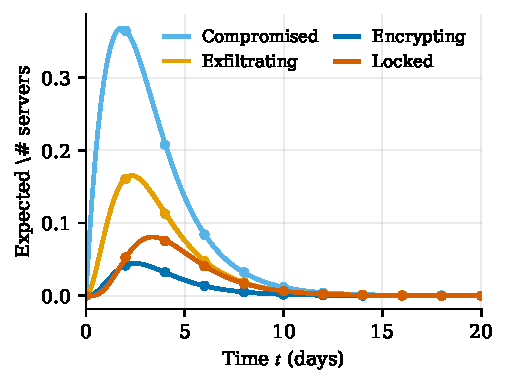
\includegraphics[width=\columnwidth]{fig01_stage_counts}
\caption{Kill-chain stage populations.}
\label{fig:stage}
\end{figure}

\begin{figure}[t]
\centering
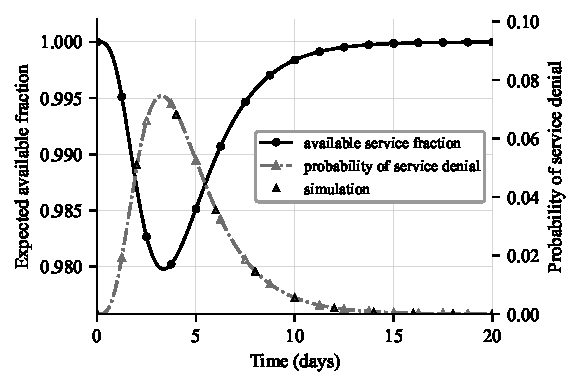
\includegraphics[width=\columnwidth]{fig02_availability}
\caption{Service availability and denial probability.}
\label{fig:avail}
\end{figure}

\subsection{Accumulated security and dependability loss}
Fig.~\ref{fig:loss} decomposes the accumulated expected loss into exfiltration,
service denial, recovery-point data loss and response components. The loss
accrues steeply during the active phase and saturates after incident resolution.
The composition across confidentiality, availability and recency tells a
defender which harm dominates and hence which lever deserves investment.

\begin{figure}[t]
\centering
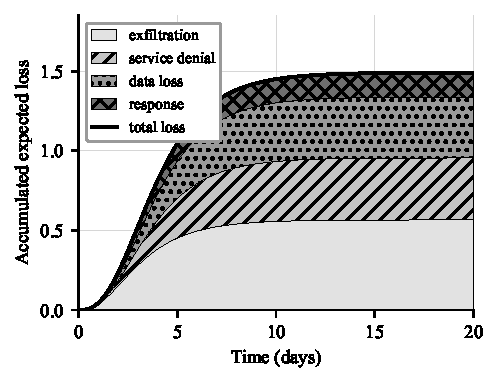
\includegraphics[width=\columnwidth]{fig03_loss_accum}
\caption{Accumulated loss decomposition.}
\label{fig:loss}
\end{figure}

\subsection{Detection race and non-memoryless recovery}
Fig.~\ref{fig:detect} shows the detection distribution function for a range of
detection sensitivities, including one degraded setting below the lower bound of
the co-design lever box. Sharper detection compresses the stealth window, and
the baseline hazard keeps the detection probability rising toward one even for a
dull monitor, because every campaign eventually generates a footprint.
Fig.~\ref{fig:resolve} carries the headline structural result of the whole
study. The resolution
curve takes a clear S shape with an initial dead time while the campaign remains
stealthy, and the curve departs from the best-fit memoryless exponential by
\Cresdev{} at the maximum. A uniform-recovery model of the
form of~\cite{liu2021transient} cannot represent such behaviour, and the
coupling of detection to attack progress makes edge ransomware resolution
non-memoryless.

\begin{figure}[t]
\centering
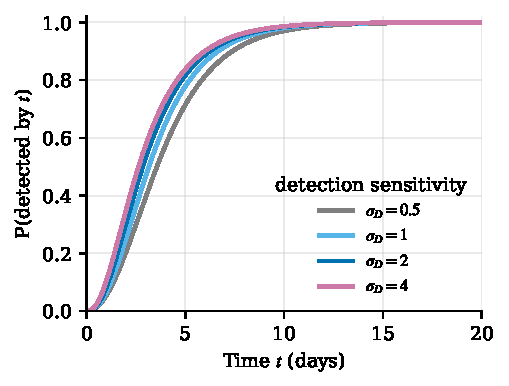
\includegraphics[width=\columnwidth]{fig04_detection_race}
\caption{Detection distribution function.}
\label{fig:detect}
\end{figure}

\begin{figure}[t]
\centering
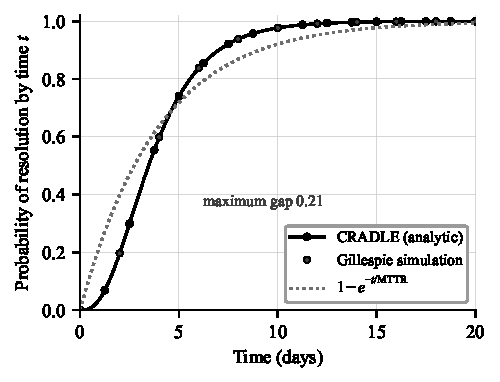
\includegraphics[width=\columnwidth]{fig05_resolution}
\caption{Resolution probability against exponential fit.}
\label{fig:resolve}
\end{figure}

\subsection{Defender co-design}
Fig.~\ref{fig:surface} maps the expected total cost over the plane of detection
sensitivity and backup cadence, and a fine grid sweep locates a single interior
basin. Cost rises steeply at short backup intervals through storage overhead and
rises more gently at high sensitivity through monitoring overhead, while very
loose backups or a dull monitor raise the security loss well above the optimum.
Algorithm~\ref{alg:codesign} locates the optimum at a sensitivity of \Csigstar{}
and a backup interval of \Ctaustar{} hours, where the security loss and the
operational spend end up nearly balanced. Fig.~\ref{fig:pareto} traces the
corresponding Pareto frontier, and the minimum-total-cost design sits at the
point where the marginal security gain equals the marginal spend.
Table~\ref{tab:codesign} contrasts the baseline, a detection-blind backup-only
optimizer, and the co-design.

\begin{figure}[t]
\centering
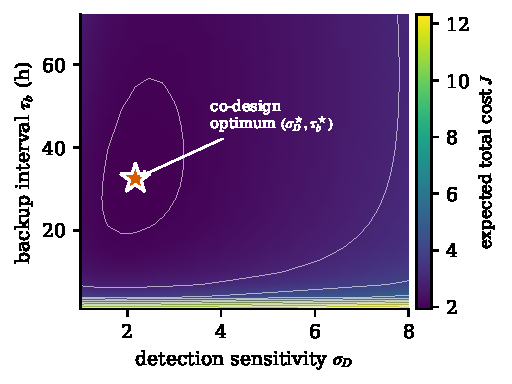
\includegraphics[width=\columnwidth]{fig06_costsurface}
\caption{Expected total cost surface.}
\label{fig:surface}
\end{figure}

\begin{figure}[t]
\centering
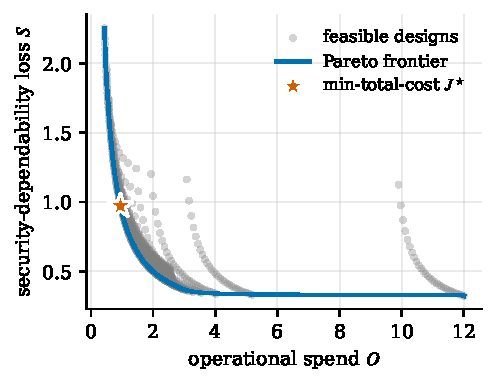
\includegraphics[width=\columnwidth]{fig07_pareto}
\caption{Security-loss and operational-spend frontier.}
\label{fig:pareto}
\end{figure}

\begin{table}[t]
\caption{Baseline, detection-blind and co-design comparison.}
\label{tab:codesign}
\centering\footnotesize
\setlength{\tabcolsep}{4pt}
\begin{tabular}{@{}lrrrrrrrr@{}}
\toprule
design & $\sigma_D$ & $\tau_b$(h) & E[exfil] & E[denial] & E[loss] & $S$ & $O$ & $J$\\
\midrule
baseline & 1.0 & 24 & 0.566 & 0.389 & 0.382 & 1.491 & 0.700 & 2.191\\
detection-blind & 1.0 & 25 & 0.566 & 0.389 & 0.382 & 1.491 & 0.691 & 2.191\\
\midrule
\textbf{co-design}~$\star$ & 2.17 & 32 & 0.385 & 0.149 & 0.296 & 0.971 & 0.947 & 1.918\\
\bottomrule
\end{tabular}

\end{table}

The counterintuitive finding lies in the levers themselves
(Figs.~\ref{fig:levsig} and \ref{fig:levtau}). A detection-blind operator cannot
reduce the number of servers reaching the locked stage, and such an operator
therefore spends more of the budget on frequent backups and nothing extra on
detection, which costs a penalty of \Cblindpen\% in total cost relative to the
co-design. The co-designer instead sharpens detection until far fewer servers
ever reach the locked stage, which cuts expected denial by \Cdenialdroppct\% and
expected data loss by \ClossDropPct\%. The co-designer can then relax the backup
interval and save storage overhead. Better detection buys looser backups,
because the two levers act as economic substitutes, and tuning the levers
independently remains strictly sub-optimal.

\begin{figure}[t]
\centering
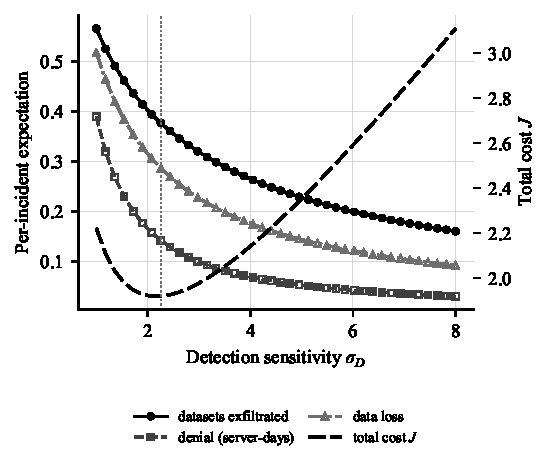
\includegraphics[width=\columnwidth]{fig08_lever_sigma}
\caption{Effect of detection sensitivity.}
\label{fig:levsig}
\end{figure}

\begin{figure}[t]
\centering
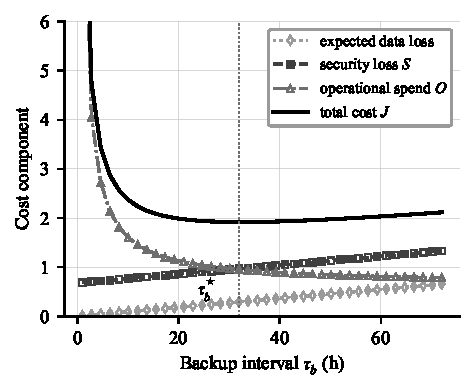
\includegraphics[width=\columnwidth]{fig09_lever_tau}
\caption{Effect of backup interval.}
\label{fig:levtau}
\end{figure}

\subsection{Fleet size and parameter sensitivity}
Fig.~\ref{fig:scaling} scales the MEDC from \CmLo{} to \CmHi{} servers, which
grows the state space from \CntLo{} to \CntHi{} transient states. The
per-incident harms saturate, because detection resolves the incident before the
campaign traverses the whole fleet, and the expected number of exfiltrated
datasets and the denial server-days barely grow with fleet size. For edge
micro-datacenters the practical message names detection latency and backup
recency as the governing factors of ransomware risk. Fig.~\ref{fig:sens} ranks the
drivers of expected data loss by scaled sensitivity. The backup recovery point
dominates with unit elasticity, the exfiltration-completion rate and the
encryption-completion rate follow, and every detection coefficient reduces the
loss, which confirms the co-design intuition. The compromised-stage detection
gain is zero at the baseline and admits no scaled sensitivity, hence the ranking
omits the coefficient.

\begin{figure}[t]
\centering
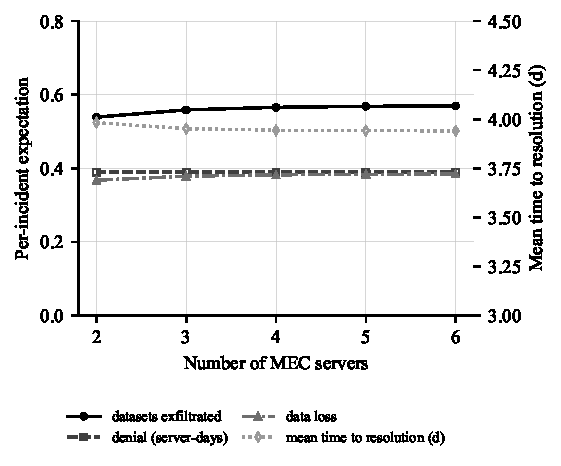
\includegraphics[width=\columnwidth]{fig10_scaling}
\caption{Per-incident measures against fleet size.}
\label{fig:scaling}
\end{figure}

\begin{figure}[t]
\centering
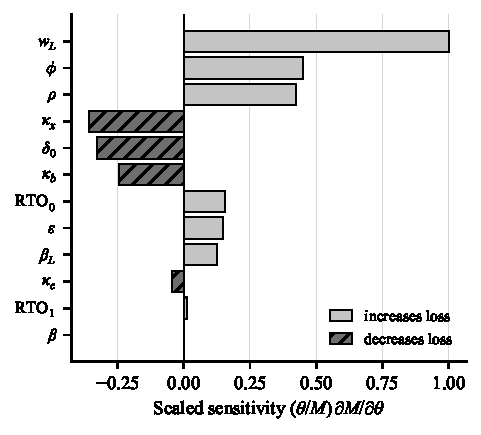
\includegraphics[width=\columnwidth]{fig11_sensitivity}
\caption{Scaled sensitivity of expected data loss.}
\label{fig:sens}
\end{figure}

\subsection{Robustness to imperfect restore}
Real restores sometimes fail to evict the adversary completely, because a
restored server can be re-infected from a missed persistence foothold, and
double-extortion crews often re-encrypt in order to punish incomplete recovery.
Fig.~\ref{fig:cov} sweeps the restore coverage from a perfect value down to 0.6.
As coverage degrades, a fraction of incidents relapse into a fresh campaign
before final resolution, and both the mean time to resolution and the expected
data loss inflate in a convex manner. The inflation reaches \CcovMttrPct\% in
resolution time and \CcovLossPct\% in data loss at a coverage of 0.7. The
practical corollary elevates restore quality, meaning a verified, immutable and
fully evicting restore, into a first-order concern, because a cheap and leaky
restore erases the benefit of an otherwise well-tuned co-design.

\begin{figure}[t]
\centering
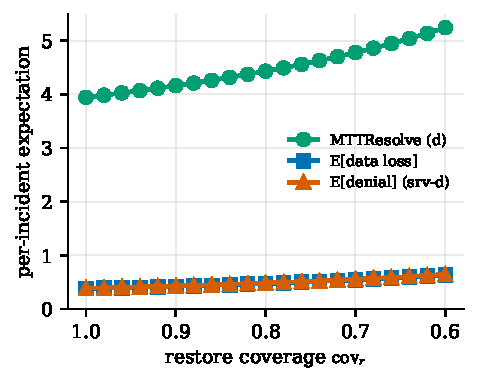
\includegraphics[width=\columnwidth]{fig12_coverage}
\caption{Robustness to imperfect restore coverage.}
\label{fig:cov}
\end{figure}

\subsection{Design guidance and threats to validity}
Three guidelines follow from the numerical study. First, instrumenting for the
crypto footprint pays best, because the detection hazard rises with encryption
input-output and tuning the monitor toward high-entropy write bursts gives the
steepest security return. Second, detection and backups deserve joint budgeting,
because the two levers act as substitutes and separate budgeting causes
over-spending.
Third, fleet size is not the dominant risk factor, because per-incident harm
saturates and consolidation for efficiency does not materially raise ransomware
exposure once detection and restore are in place.

Several modelling assumptions bound the scope of the present study. CRADLE assumes exponential
stage sojourns, and heavy-tailed encryption or restore times need a semi-Markov
or phase-type refinement, which the accumulated-reward and fundamental-matrix
machinery accommodates directly. We assume incorruptible immutable backups and
effective isolation, and relaxing the two assumptions adds arcs without new
formalism. The cost weights are illustrative, the framework consumes any
weights, and the qualitative guidance on lever substitutability and on
saturation with fleet size stayed stable across the sweeps of the study.
Finally, the ransom-payment game falls outside the scope by design, because
CRADLE models the resilience of a restore-not-pay defender.

% ======================================================================= %
\section{Conclusion}\label{sec:concl}
The study presented CRADLE, a transient stochastic-reward-net model of a
crypto-ransomware double-extortion kill-chain on a MEC micro-datacenter,
defended by a footprint-aware endpoint monitor and by an immutable-backup
isolate-and-restore response. Unlike prior edge-under-attack models, CRADLE
treats encryption as a recoverable service-denial state rather than an absorbing
breach, orders exfiltration before encryption in order to capture double
extortion, ties the detection hazard to the encryption and exfiltration
footprint, and endows the response with explicit recovery-point and
recovery-time economics. From one generator we obtained transient stage and
service-denial probabilities, accumulated-reward losses in confidentiality,
availability and data recency, first-passage detection and resolution
distributions, and closed per-incident expectations through the fundamental
matrix. We proved and demonstrated a qualitative departure from uniform-recovery
models, because coupling detection to attack progress makes the resolution law
non-memoryless. A co-design procedure tuned detection sensitivity and
backup cadence jointly to minimize expected total cost, revealed a Pareto
frontier and the substitutability of the two levers, under which sharper
detection lets a defender back up less often, while per-incident harm saturates
with fleet size. An independent exact simulation validated every analytic
result of the whole study. Future work lifts the exponential assumption toward semi-Markov
sojourns for heavy-tailed encryption and restore times, embeds an adaptive
state-triggered response policy, extends the model to federations of interacting
micro-datacenters, and incorporates the strategic ransom-payment decision as a
game against the modeled defender.

% ======================================================================= %
\begin{thebibliography}{99}
\footnotesize

\bibitem{mao2017survey} Y.~Mao, C.~You, J.~Zhang, K.~Huang, and K.~B.~Letaief,
``A survey on mobile edge computing: The communication perspective,''
\emph{IEEE Commun. Surveys Tuts.}, vol.~19, no.~4, pp.~2322--2358, 2017,
doi: 10.1109/COMST.2017.2745201.

\bibitem{taleb2017mec} T.~Taleb, K.~Samdanis, B.~Mada, H.~Flinck, S.~Dutta, and
D.~Sabella, ``On multi-access edge computing: A survey of the emerging 5G
network edge cloud architecture and orchestration,'' \emph{IEEE Commun. Surveys
Tuts.}, vol.~19, no.~3, pp.~1657--1681, 2017,
doi: 10.1109/COMST.2017.2705720.

\bibitem{roman2018survey} R.~Roman, J.~Lopez, and M.~Mambo, ``Mobile edge
computing, Fog et al.: A survey and analysis of security threats and
challenges,'' \emph{Future Gener. Comput. Syst.}, vol.~78, pp.~680--698, 2018,
doi: 10.1016/j.future.2016.11.009.

\bibitem{kharraz2015gordian} A.~Kharraz, W.~Robertson, D.~Balzarotti,
L.~Bilge, and E.~Kirda, ``Cutting the Gordian knot: A look under the hood of
ransomware attacks,'' in \emph{Proc. DIMVA}, LNCS 9148, 2015, pp.~3--24,
doi: 10.1007/978-3-319-20550-2\_1.

\bibitem{alrimy2018ransomware} B.~A.~S.~Al-rimy, M.~A.~Maarof, and
S.~Z.~M.~Shaid, ``Ransomware threat success factors, taxonomy, and
countermeasures: A survey and research directions,'' \emph{Comput. Secur.},
vol.~74, pp.~144--166, 2018, doi: 10.1016/j.cose.2018.01.001.

\bibitem{razaulla2023age} S.~Razaulla, C.~Fachkha, C.~Markarian, A.~Gawanmeh,
W.~Mansoor, B.~C.~M.~Fung, and C.~Assi, ``The age of ransomware: A survey on the
evolution, taxonomy, and research directions,'' \emph{IEEE Access}, vol.~11,
pp.~40698--40723, 2023, doi: 10.1109/ACCESS.2023.3268535.

\bibitem{beaman2021ransomware} C.~Beaman, A.~Barkworth, T.~D.~Akande, S.~Hakak,
and M.~K.~Khan, ``Ransomware: Recent advances, analysis, challenges and future
research directions,'' \emph{Comput. Secur.}, vol.~111, art.~102490, 2021,
doi: 10.1016/j.cose.2021.102490.

\bibitem{continella2016shieldfs} A.~Continella, A.~Guagnelli, G.~Zingaro,
G.~De~Pasquale, A.~Barenghi, S.~Zanero, and F.~Maggi, ``ShieldFS: A
self-healing, ransomware-aware filesystem,'' in \emph{Proc. ACSAC}, 2016,
pp.~336--347, doi: 10.1145/2991079.2991110.

\bibitem{kharraz2017redemption} A.~Kharraz and E.~Kirda, ``Redemption:
Real-time protection against ransomware at end-hosts,'' in \emph{Proc. RAID},
LNCS 10453, 2017, pp.~98--119, doi: 10.1007/978-3-319-66332-6\_5.

\bibitem{gazet2010comparative} A.~Gazet, ``Comparative analysis of various
ransomware virii,'' \emph{J. Comput. Virol.}, vol.~6, no.~1, pp.~77--90, 2010,
doi: 10.1007/s11416-008-0092-2.

\bibitem{sood2013crimeware} A.~K.~Sood and R.~J.~Enbody, ``Crimeware-as-a-service:
A survey of commoditized crimeware in the underground market,'' \emph{Int. J.
Crit. Infrastruct. Prot.}, vol.~6, no.~1, pp.~28--38, 2013,
doi: 10.1016/j.ijcip.2013.01.002.

\bibitem{ussath2016apt} M.~Ussath, D.~Jaeger, F.~Cheng, and C.~Meinel,
``Advanced persistent threats: Behind the scenes,'' in \emph{Proc. CISS}, 2016,
pp.~181--186, doi: 10.1109/CISS.2016.7460498.

\bibitem{liu2021transient} B.~Liu, A.~Bobbio, J.~Bai, J.~Martinez, X.~Chang,
and K.~S.~Trivedi, ``Transient security and dependability analysis of MEC micro
datacenter under attack,'' in \emph{Proc. Annu. Rel. Maintainab. Symp. (RAMS)},
2021, pp.~1--7, doi: 10.1109/RAMS48097.2021.9605723.

\bibitem{trivedi2016probability} K.~S.~Trivedi, \emph{Probability and Statistics
with Reliability, Queuing, and Computer Science Applications}, 2nd~ed. Hoboken,
NJ, USA: Wiley, 2016, doi: 10.1002/9781119285441.

\bibitem{trivedi2017reliability} K.~S.~Trivedi and A.~Bobbio, \emph{Reliability
and Availability Engineering: Modeling, Analysis, and Applications}. Cambridge,
U.K.: Cambridge Univ. Press, 2017, doi: 10.1017/9781316163047.

\bibitem{meyer1980performability} J.~F.~Meyer, ``On evaluating the
performability of degradable computing systems,'' \emph{IEEE Trans. Comput.},
vol.~C-29, no.~8, pp.~720--731, 1980, doi: 10.1109/TC.1980.1675654.

\bibitem{nicol2004modelbased} D.~M.~Nicol, W.~H.~Sanders, and K.~S.~Trivedi,
``Model-based evaluation: From dependability to security,'' \emph{IEEE Trans.
Dependable Secure Comput.}, vol.~1, no.~1, pp.~48--65, 2004,
doi: 10.1109/TDSC.2004.11.

\bibitem{ciardo1992srn} G.~Ciardo, J.~K.~Muppala, and K.~S.~Trivedi,
``Analyzing concurrent and fault-tolerant software using stochastic reward
nets,'' \emph{J. Parallel Distrib. Comput.}, vol.~15, no.~3, pp.~255--269, 1992,
doi: 10.1016/0743-7315(92)90007-A.

\bibitem{madan2004method} B.~B.~Madan, K.~Go\v{s}eva-Popstojanova,
K.~Vaidyanathan, and K.~S.~Trivedi, ``A method for modeling and quantifying the
security attributes of intrusion tolerant systems,'' \emph{Perform. Eval.},
vol.~56, no.~1--4, pp.~167--186, 2004, doi: 10.1016/j.peva.2003.07.008.

\bibitem{avizienis2004basic} A.~Avi\v{z}ienis, J.-C.~Laprie, B.~Randell, and
C.~Landwehr, ``Basic concepts and taxonomy of dependable and secure computing,''
\emph{IEEE Trans. Dependable Secure Comput.}, vol.~1, no.~1, pp.~11--33, 2004,
doi: 10.1109/TDSC.2004.2.

\bibitem{jajodia2011mtd} S.~Jajodia, A.~K.~Ghosh, V.~Swarup, C.~Wang, and
X.~S.~Wang, Eds., \emph{Moving Target Defense: Creating Asymmetric Uncertainty
for Cyber Threats}. New York, NY, USA: Springer, 2011,
doi: 10.1007/978-1-4614-0977-9.

\bibitem{huang1995rejuvenation} Y.~Huang, C.~Kintala, N.~Kolettis, and
N.~D.~Fulton, ``Software rejuvenation: Analysis, module and applications,'' in
\emph{Proc. FTCS}, 1995, pp.~381--390, doi: 10.1109/FTCS.1995.466961.

\bibitem{keeton2004framework} K.~Keeton and A.~Merchant, ``A framework for
evaluating storage system dependability,'' in \emph{Proc. Int. Conf. Dependable
Syst. Netw. (DSN)}, 2004, pp.~877--886, doi: 10.1109/DSN.2004.1311958.

\bibitem{reibman1988transient} A.~Reibman and K.~S.~Trivedi, ``Numerical
transient analysis of Markov models,'' \emph{Comput. Oper. Res.}, vol.~15,
no.~1, pp.~19--36, 1988, doi: 10.1016/0305-0548(88)90026-3.

\bibitem{vanloan1978} C.~Van~Loan, ``Computing integrals involving the matrix
exponential,'' \emph{IEEE Trans. Autom. Control}, vol.~23, no.~3, pp.~395--404,
1978, doi: 10.1109/TAC.1978.1101743.

\bibitem{moler2003nineteen} C.~Moler and C.~Van~Loan, ``Nineteen dubious ways to
compute the exponential of a matrix, twenty-five years later,'' \emph{SIAM
Rev.}, vol.~45, no.~1, pp.~3--49, 2003, doi: 10.1137/S00361445024180.

\bibitem{latouche1999matrix} G.~Latouche and V.~Ramaswami, \emph{Introduction to
Matrix Analytic Methods in Stochastic Modeling}. Philadelphia, PA, USA: SIAM,
1999, doi: 10.1137/1.9780898719734.

\bibitem{gillespie1977exact} D.~T.~Gillespie, ``Exact stochastic simulation of
coupled chemical reactions,'' \emph{J. Phys. Chem.}, vol.~81, no.~25,
pp.~2340--2361, 1977, doi: 10.1021/j100540a008.

\end{thebibliography}

\end{document}
